\documentclass[11pt]{beamer}

\usepackage{hyperref}
\usepackage{graphicx}

\addtobeamertemplate{navigation symbols}{%
    \usebeamerfont{footline}%
    \usebeamercolor[fg]{footline}%
    \hspace{1em}%
	\raisebox{1.2pt}[0pt][0pt]{\insertframenumber/\inserttotalframenumber}
}

\title{\Huge Vim Magic}
\subtitle{\Large Tejas Sanap}
\author{
\includegraphics[width=0.2\textwidth]{Vimlogo.png}}
\date{\small 21st September, 2019}

\begin{document}
	\begin{frame}
		\titlepage
	\end{frame}
	\begin{frame}
		\tableofcontents
	\end{frame}
	\begin{frame}{RTFM}
		\Huge READ THE FINE MANUAL.
	\end{frame}

	\section{Introduction}

		\begin{frame}
			\setcounter{framenumber}{1}
			\frametitle{A little bit of history}
			\begin{itemize}
				\item \texttt{vi} was created by Bill Joy as a full-screen extension of \texttt{em} which was a modified version of \texttt{ed}.
				\item \texttt{ed} is one of first parts of the Unix system to be developed.
				\item Later, \texttt{vi} was re-written into a much improved version, called \texttt{vim}, by Bram Moonlear.
				\item The latest iteration, is called \texttt{neovim}, which is a refactoring of the original vim.
				\item There are other interesting projects such as \texttt{onivim}, which are bringing \texttt{neovim} to the desktop, but in a very appealing manner.
			\end{itemize}
		\end{frame}

		\begin{frame}{Install \texttt{vim}}
			\begin{block}{Debian}
				\texttt{sudo add-apt-repository ppa:jonathonf/vim} \\
				\texttt{sudo apt-get update}
			\end{block}
			\begin{block}{Fedora}
				\texttt{sudo dnf install vim-enhanced gvim} 
			\end{block}
		\end{frame}

		\begin{frame}{Difference between \texttt{vi} and \texttt{vim}}
			\begin{enumerate}
				\item \texttt{vi} has limited undo history.
				\item \texttt{vi} has no syntax highlighting.
				\item \texttt{vim} has \texttt{Vimscript} support.
			\end{enumerate}
			\begin{block}{Command}
				\texttt{:help vi-differences}
			\end{block}
		\end{frame}

		\begin{frame}{Terminology}
			\begin{enumerate}
				\item Commands - \texttt{:help}
				\item Keystrokes - \texttt{<F1>}
				\item \hyperlink{https://vim.fandom.com/wiki/Vim_buffer_FAQ}{Buffers}
				\item ``Tab"page
				\item Windows/Splits
				\item Modes
			\end{enumerate}	
		\end{frame}

	\section{Modes}

		\begin{frame}{What is a modal editor?}
			\begin{enumerate}
				\item In a modal editor, the same keys have different meanings depending on the mode.
				\item This means, that the same keys can achieve more tasks.
				\item This also means, that you save keystrokes.
			\end{enumerate}
		\end{frame}

		\begin{frame}{Is vim a language? Yes.}
			\begin{itemize}
				\item \texttt{vim} treats text as \emph{text-objects} and commands perform \emph{actions} over these \emph{text-objects}.
				\item A \emph{text-object} may be a word, a paragraph, etc.
				\item An \emph{action} may be delete, change, etc.
				\item The action maybe performed inside two text objects, or around one object, or surrounding a text-object.
			\end{itemize}
			
			\begin{block}{Examples}
				\begin{center}
					\Huge d w \\
					\tiny delete \; word
				\end{center}
			\end{block}
		\end{frame}

		\subsection{Normal}
			\begin{frame}{Normal Mode}
				\only<1>{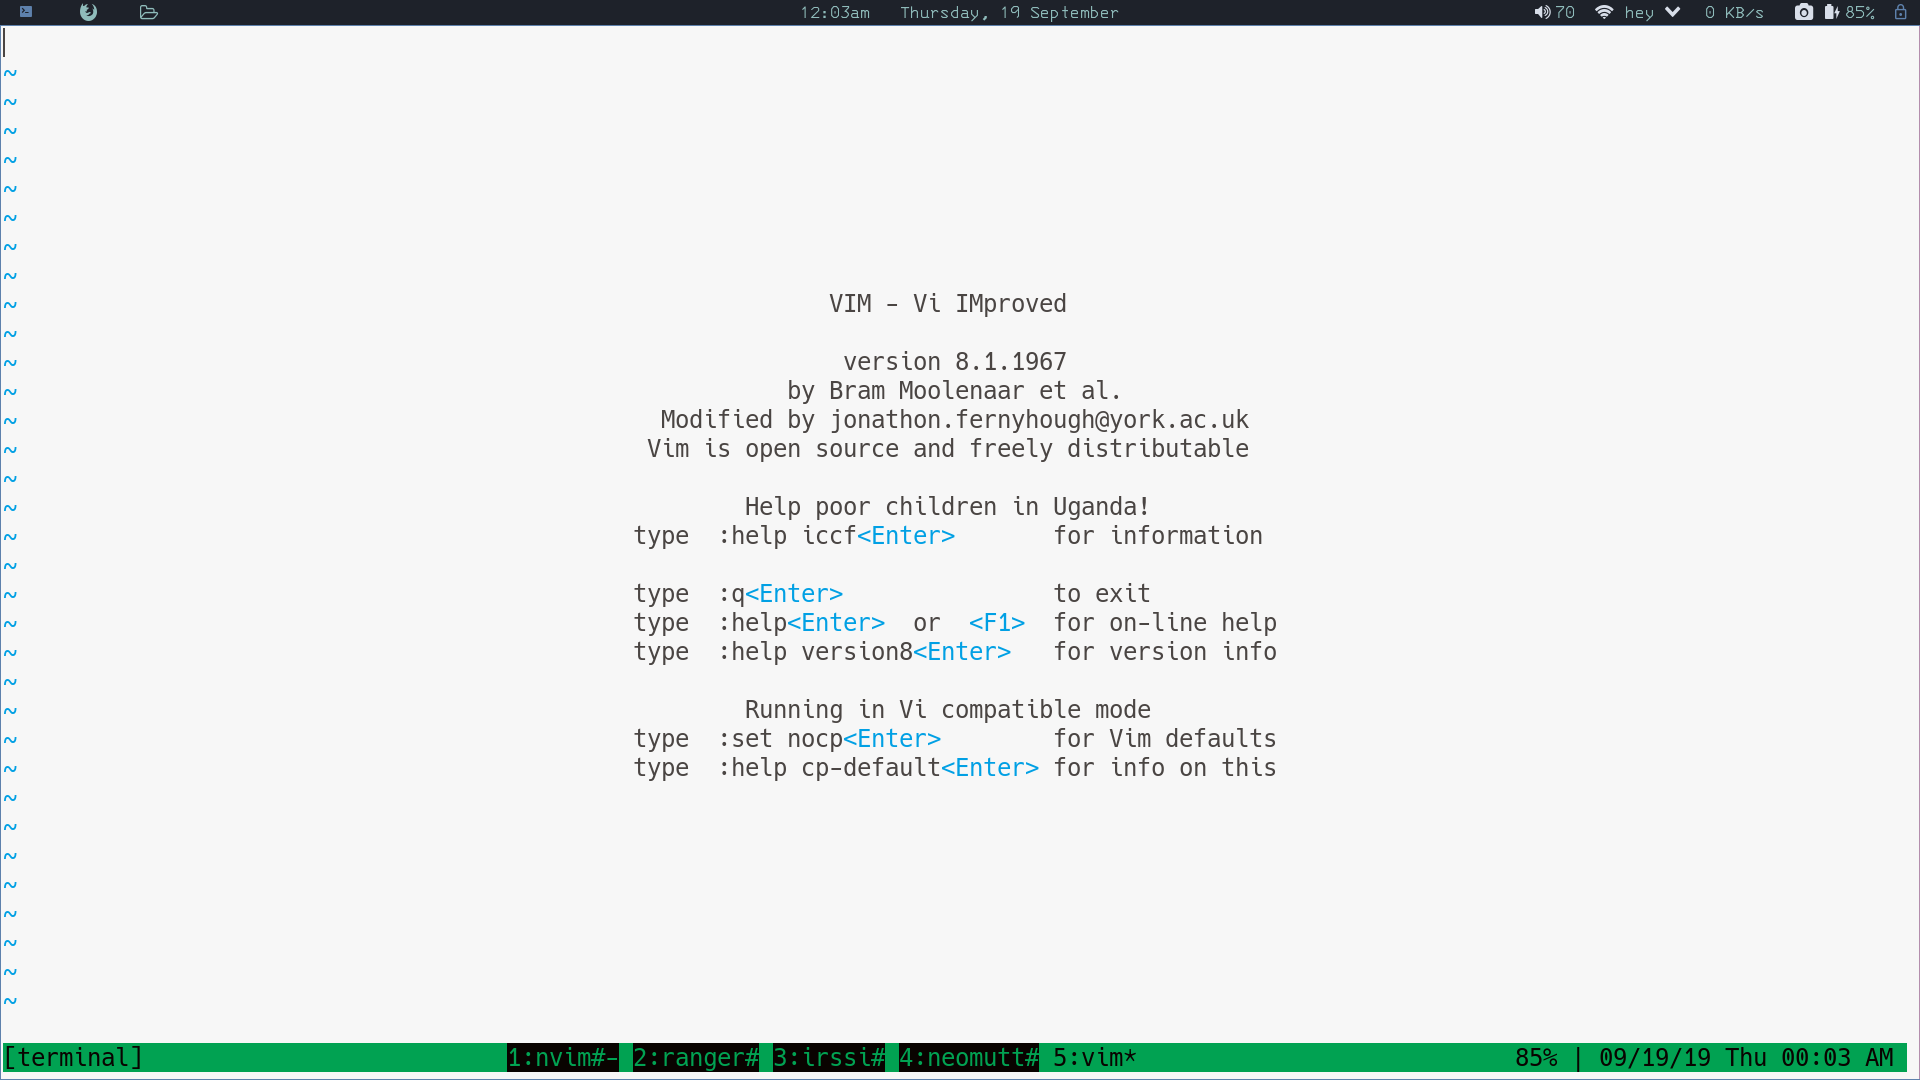
\includegraphics[width=\textwidth]{landing-page.png}}
				\only<2>{
				\begin{enumerate}
					\item \texttt{vim} always opens up in this mode.
					\item Normally, stay here.
					\item This mode is used to:
						\begin{enumerate}[i]
							\item Navigate through files.
							\item To copy and paste.
							\item To delete.
						\end{enumerate}
					\item Copy and paste in \texttt{vim} is known as:
						\begin{enumerate}
							\item Copy - Yank (\texttt{y})
							\item Paste - Put (\texttt{p})
						\end{enumerate}
				\end{enumerate}
				}
			\end{frame}

			\begin{frame}{How to navigate through a file}
				\begin{enumerate}
					\item{\textbf{Move along words}} - \texttt{w, b, e, f, t, F, T}
					\item{\textbf{Scroll}} - \texttt{<C-d>, <C-u>, <C-f>, <C-b>, <C-e>, <C-y>}
					\item{\textbf{Move the current line}} - \texttt{zt, zb, zz}
					\item{\textbf{Jump across the screen}} - \texttt{H, M, L}
				\end{enumerate}			
				\begin{block}{Command}
					\texttt{:help usr\_03.txt}
				\end{block}
			\end{frame}

		\subsection{Insert}
			\begin{frame}{Insert Mode}
				\only<1>{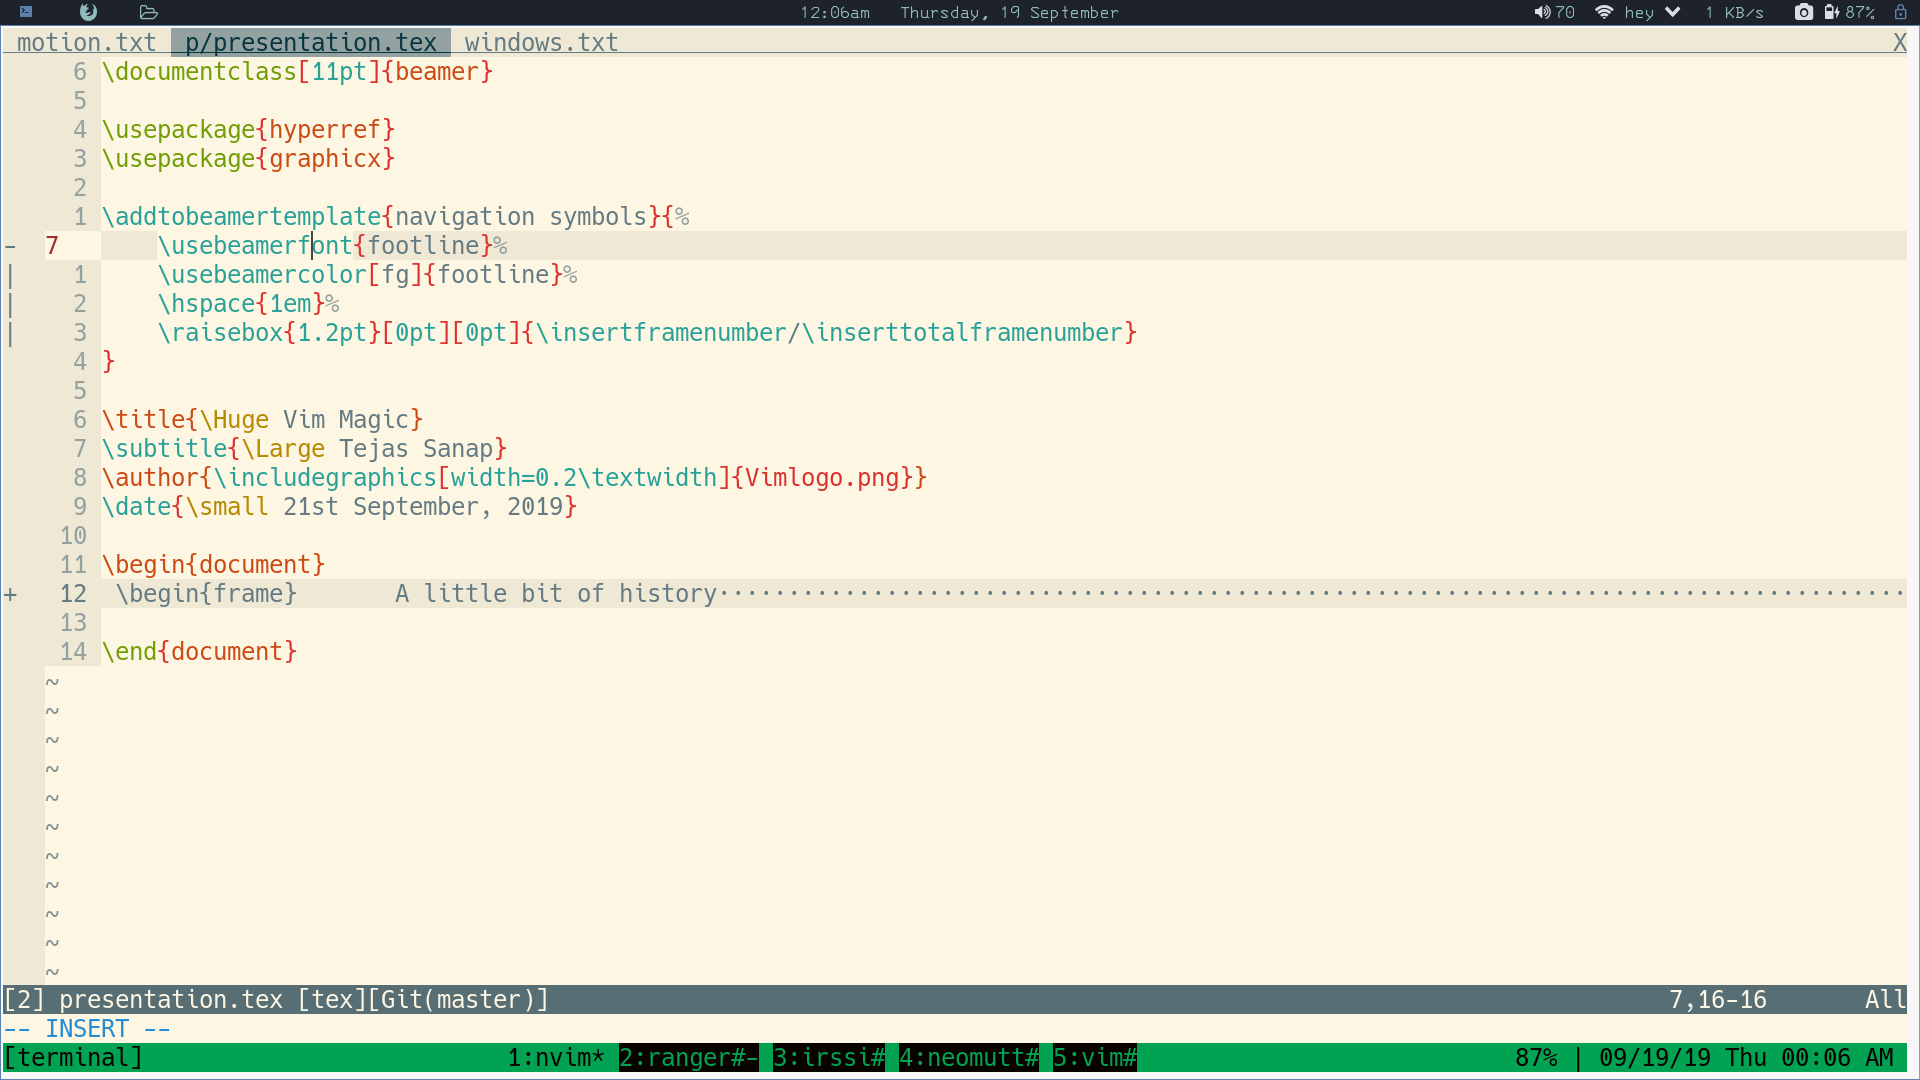
\includegraphics[width=\textwidth]{insert-mode.png}}
				\only<2>{
				\begin{enumerate}
					\item Only jump in here, when necessary.
					\item Enter insert mode in short bursts.
					\item \texttt{vim} offers text-completion from various sources.
				\end{enumerate}
				\begin{block}{Command}
					\texttt{:help usr\_24.txt}
				\end{block}
				}
			\end{frame}

		\subsection{Visual}
			\begin{frame}{Visual Mode}
				\begin{enumerate}
					\item Visual mode is a great help during yank/put operations.
					\item Has \textbf{three} modes:
						\begin{enumerate}[i]
							\item visual mode per character - \texttt{v}
							\item visual mode linewise - \texttt{<S-v>}
							\item visual mode blockwise - \texttt{<C-v>}
						\end{enumerate}
				\end{enumerate}
				\begin{block}{Command}
					\texttt{:help visual.txt}
				\end{block}
			\end{frame}

	\section{Tabs and Splits}
		
		\begin{frame}{Splits}
			\begin{enumerate}
				\item Divide the current window into splits, producing two viewports.
				\item Splits can be vertical and horizontal.
			\end{enumerate}
			\begin{center}
				\only<1>{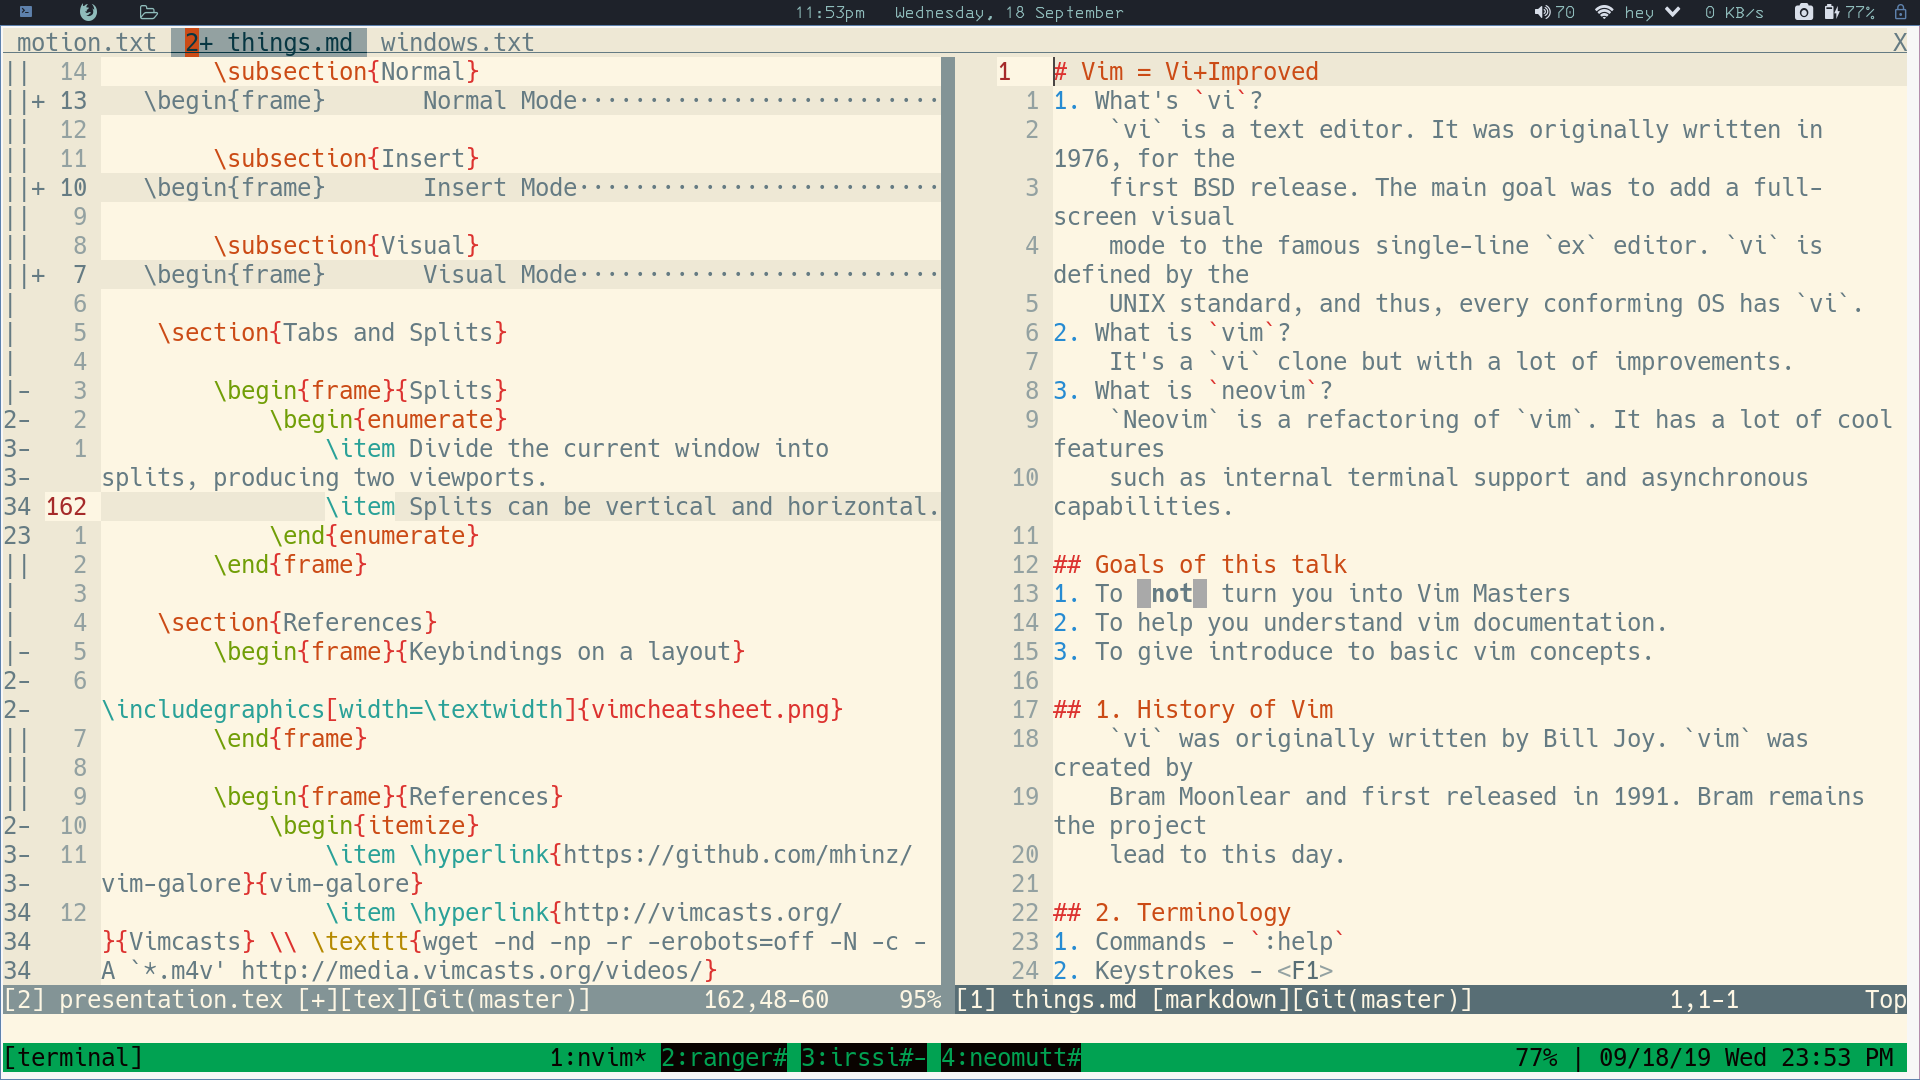
\includegraphics[width=0.9\textwidth]{split1.png}}
				\only<2>{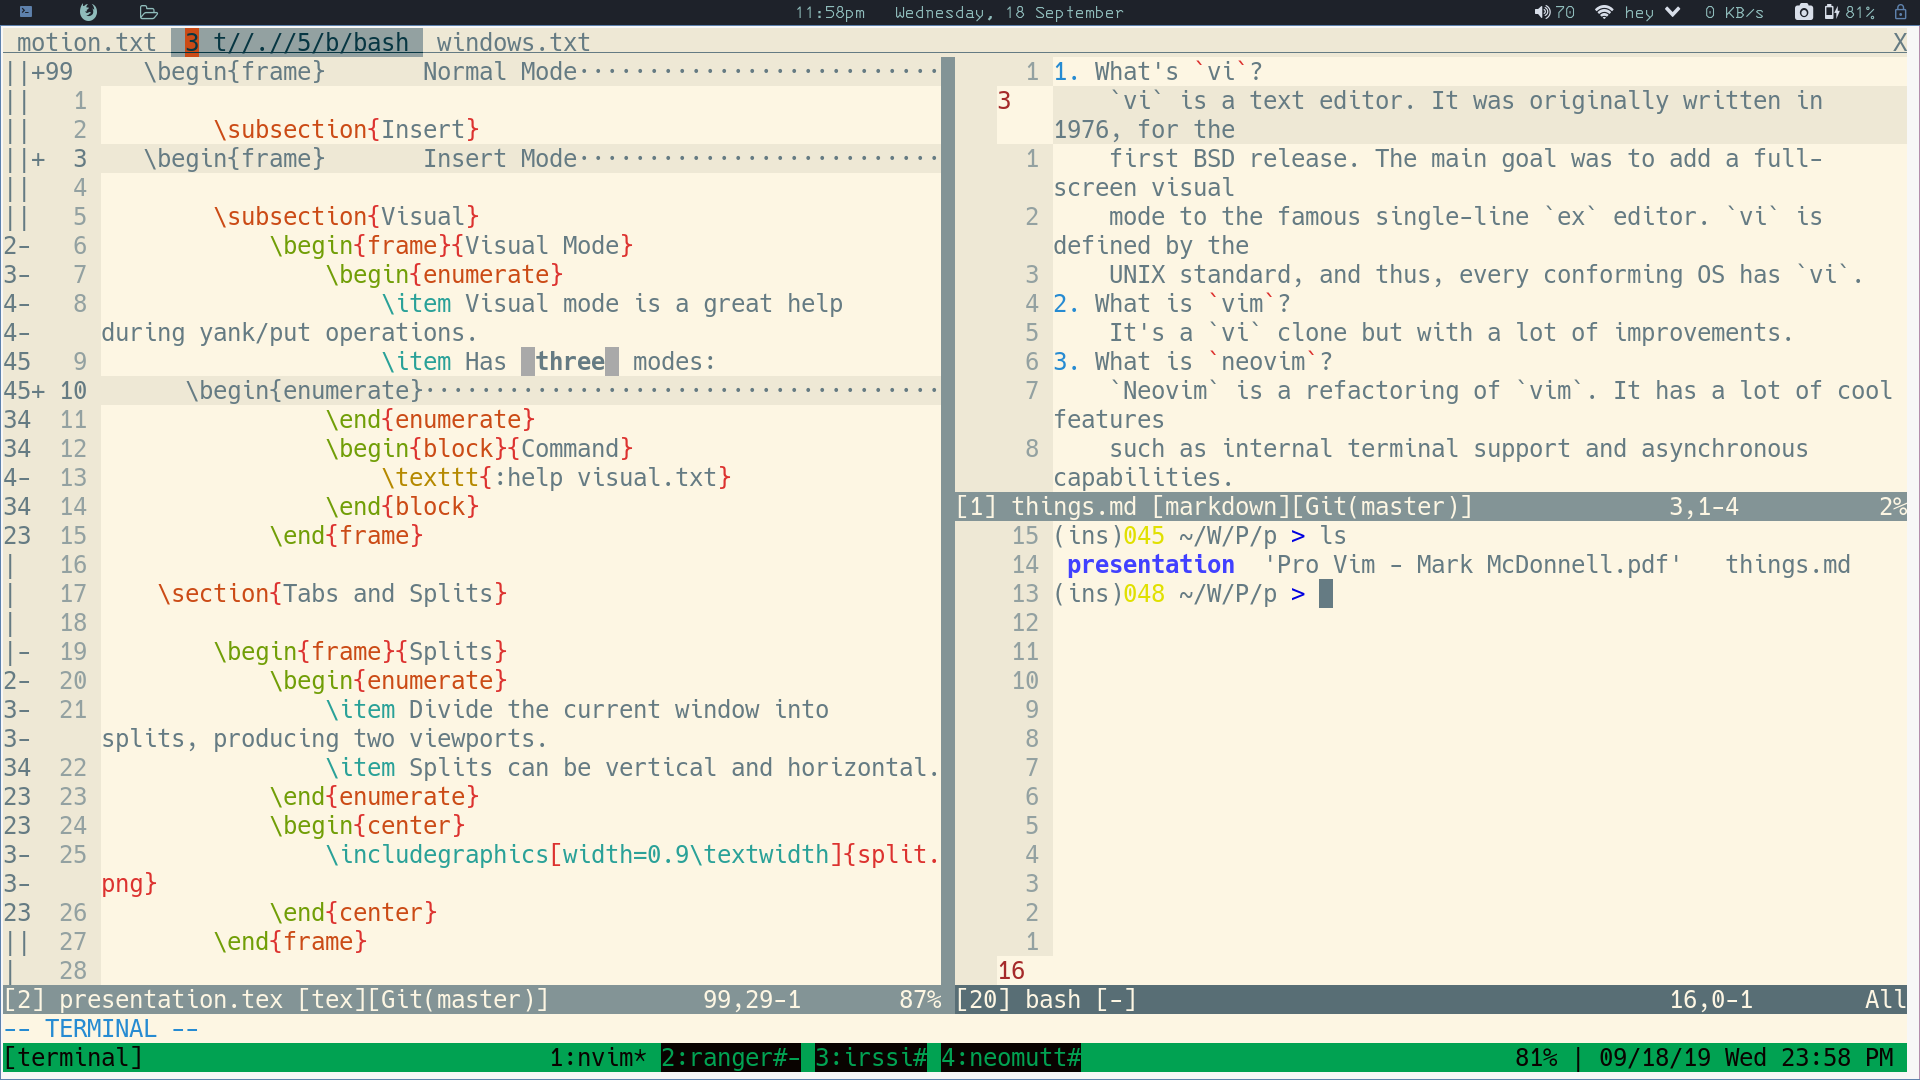
\includegraphics[width=0.9\textwidth]{split2.png}}
			\end{center}
		\end{frame}

		\subsection{Manage your splits}

			\begin{frame}{Manage your splits}
				\begin{block}{Command}
					\texttt{:help Q\_wi}
				\end{block}
			\end{frame}

		\subsection{Manage your tabs}

			\begin{frame}{Manage your tabs}
				\begin{block}{Command}
					\texttt{:help tabpage.txt}
				\end{block}
			\end{frame}
	
	\section{Auto-complete}
		
		\begin{frame}{Insert-completion mode}
			\begin{block}{Command}
				\texttt{:help ins-completion} \\
				\texttt{:help ins-completion-menu}
			\end{block}
		\end{frame}

	\section{Mappings}
		
		\begin{frame}{Remapping? What is this?}
			It's magic!
			\begin{block}{Command}
				\texttt{:help map.txt}
			\end{block}
		\end{frame}

	\section{Registers}
	
		\begin{frame}{Registers}
			Does your copy-paste thingy not work? Don't worry we have got you covered?
			\begin{block}{Command}
				\texttt{:help registers}
			\end{block}
		\end{frame}

	\section{Show us some cool tricks!}

		\subsubsection{Expression Register}
		
		\begin{frame}{The in-built calculator}
			The \texttt{=} register.
		\end{frame}

		\subsubsection{Use external commands}

		\begin{frame}{Format emails}
			\begin{block}{Command}
				\texttt{!fmt -w 72}
			\end{block}
		\end{frame}

	\section{References}

		\begin{frame}{Keybindings on a layout}
			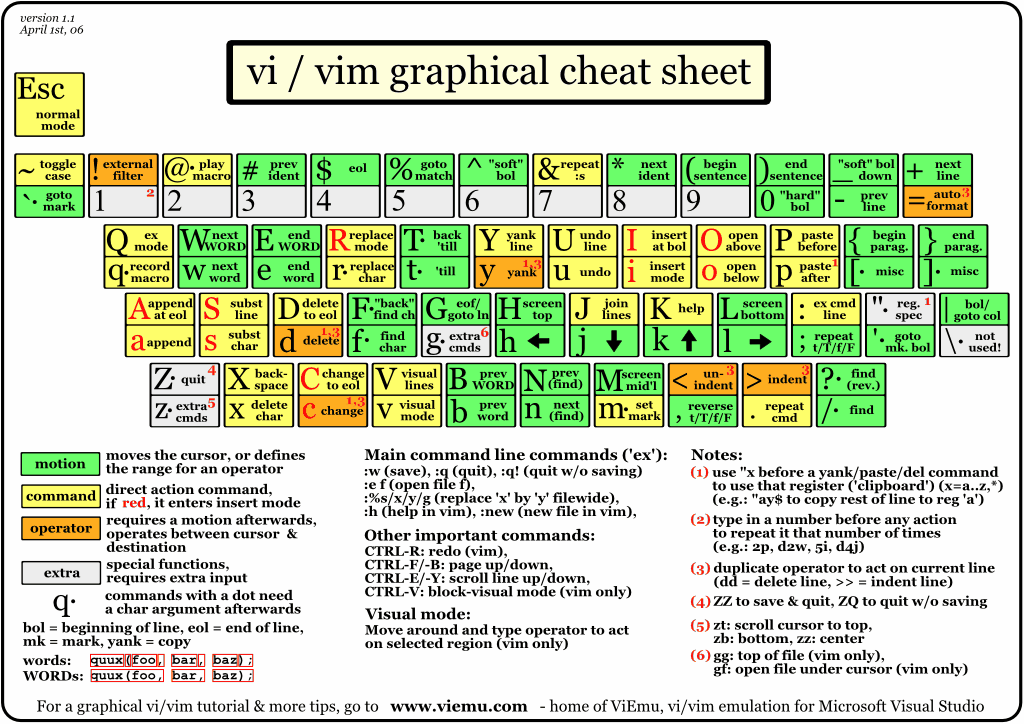
\includegraphics[width=\textwidth]{vimcheatsheet.png}
		\end{frame}

		\begin{frame}{References}
			\begin{itemize}
				\item \hyperlink{https://github.com/mhinz/vim-galore}{vim-galore}
				\item \hyperlink{http://vimcasts.org/}{Vimcasts} \\ \texttt{wget -nd -np -r -erobots=off -N -c -A `*.m4v' http://media.vimcasts.org/videos/}
				\item Thoughtbot on Youtube
			\end{itemize}	
		\end{frame}

		\begin{frame}{Questions?}
			\hyperlink{https://whereistejas.me}{whereistejas.me} \\
			\hyperlink{mailto:sanap.tejas@gmail.com}{sanap.tejas@gmail.com} \\
			IRC nick: whereistejas \\
		\end{frame}

\end{document}
